\newpage

\section{Detekcja oczu} \label{section:eye_detection}

Przed przystąpieniem do detekcji oczu należy wyznaczyć obszar, na którym wykryta została twarz (patrz rozdz. \hyperref[{section:face_detection}]{\textit{\ref{section:face_detection}.Detekcja twarzy}}).
\\
Następnie obcinając klatkę tylko do ustalonego prostokąta wykrywam oczy za pomocą \textit{Cascading Classifier} - podobnie jak twarz.
---------- to będzie usunięte jeśli dam więcej algorytmów ------------

Wynik który chcę uzyskać - wykryte oczy powinny się znaleźć pomiędzy naniesionymi prostkątami:
-------- to będzie przeniesione do badania ewentualnie, jeśli dam więcej algorytmów ------------

\begin{figure}[!h]
    \begin{center}
        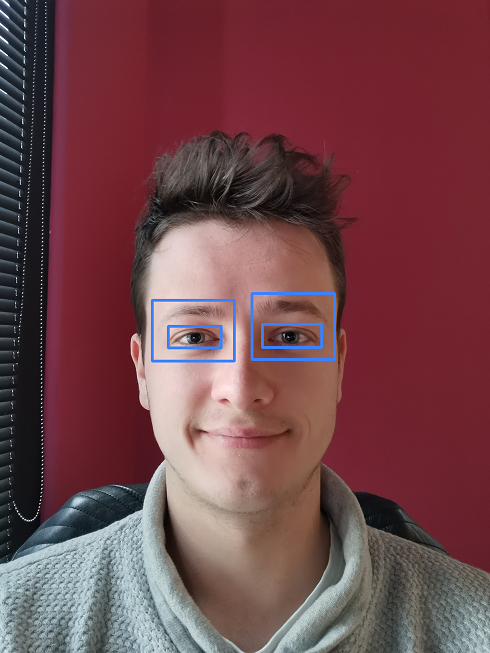
\includegraphics[scale=0.6]{img/pupil_section/expected_eyes_region.png}
        \caption{Przybliżony obszar oczu, który chcę wykrywać}
        \label{fig:expected_eyes_region}
    \end{center}
\end{figure}

\subsection{Obcięcie obszaru detekcji}
Dodatkowo - prócz detekcji jedynie na obszarze twarzy - zdecydowałem się zawęzić płaszczyznę przeszukiwań.
Wstępnie metodą prób i błędów dobrałem następujące parametry obcięcia obszaru:
\begin{itemize}
    \item Góra: $0.1$
    \item Dół: $0.45$
    \item Lewo: $0.1$
    \item Prawo: $0.1$
\end{itemize}

Parametr określa jaka część obszaru zostaje pominięta z poszczególnych stron. Wynik takiego obcięcia widoczny jest na \hyperref[{fig:eye_crop}]{\textit{rysunku \ref{fig:eye_crop}}}.

\begin{figure}[!h]
    \begin{center}
        \subfigure[Wykryty obszar twarzy]{\label{fig:eye_crop_before}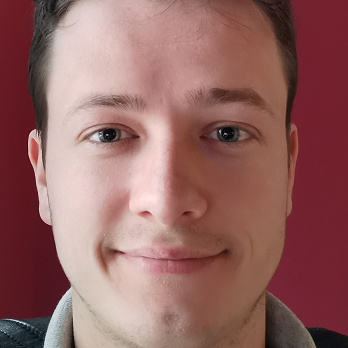
\includegraphics[scale=0.6]{img/eye_section/eye_cropped_face.png}}
        \hspace{8mm}
        \subfigure[Wycięty obszar oczu]{\label{fig:eye_crop_after}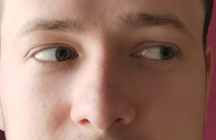
\includegraphics[scale=0.6]{img/eye_section/eye_cropped_eyes.png}}
    \end{center}
    \caption{Obcięcie obszaru detekcji oczu zgodnie z dobranymi wcześniej parametrami}
    \label{fig:eye_crop}
\end{figure}

Takie zawężenie obszaru detekcji pozwoliło wyeliminować cześć z błędnie oznaczonych oczu. Na \hyperref[{fig:eye_crop}]{\textit{rysunku \ref{fig:eye_crop}}} widoczne są dodatkowe wykryte obszary oraz ich odrzucenie dzięki temu przekształceniu.

\begin{figure}[!h]
    \begin{center}
        \subfigure[Wykrywanie oczu bez dodatkowego obcięcia obszaru]{\label{fig:eye_detect_crop_before}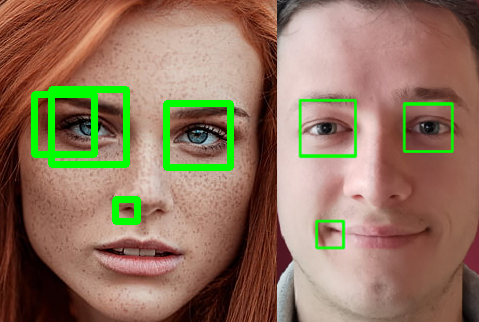
\includegraphics[scale=0.45]{img/eye_section/eye_detect_before_crop_1.png}}
        \hspace{8mm}
        \subfigure[Wykrywanie oczu z dodatkowym obcięciem obszaru]{\label{fig:eye_detect_crop_after}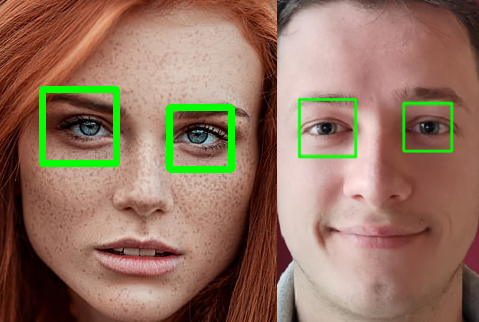
\includegraphics[scale=0.45]{img/eye_section/eye_detect_after_crop_1.png}}
    \end{center}
    \caption{Odrzucenie błędnych rezultatów detekcji oczu po dodatkowym obcięciu obszaru. Źródło pierwszego zdj.:\cite{readheadPortrait2}}
    \label{fig:eye_detect_crop}
\end{figure}

{\_\_\_\_} przyszłości zrobić testy na wielu zdjęciach wraz z wynikami przed/po w formie liczbowej. Wtedy dobrać testowo nowe parametry {\_\_\_\_}

\subsection{Filtrowanie wyników}

Ze względu na możliwość błędnych wskazań wprowadziłem filtrowanie wyników detekcji oczu. \\
Algorytm filtrowania składa się z dwóch etapów:

\begin{itemize}
    \item Podzielenie wykrytych obszarów na dwie grupy - na lewą i prawą stronę twarzy
    \item W obu grup wybranie największego obszaru
\end{itemize}

Przykład rezultatu takiego filtrowania pokazany jest na \hyperref[{fig:eye_filter}]{\textit{rysunku \ref{fig:eye_filter}}}. Dodatkowo pozwoliło to na łatwe zidentyfikowanie który obszar to które oko i ich posortowanie.

\begin{figure}[!h]
    \begin{center}
        \subfigure[Przed filtrowaniem]{\label{fig:eye_filter_before}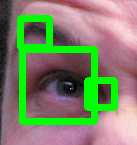
\includegraphics[scale=1.0]{img/eye_section/eye_filter_before.png}}
        \hspace{8mm}
        \subfigure[Po filtrowaniu]{\label{fig:eye_filter_after}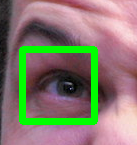
\includegraphics[scale=1.0]{img/eye_section/eye_filter_after.png}}
    \end{center}
    \caption{Efekt filtrowania obszarów detekcji oczu}
    \label{fig:eye_filter}
\end{figure}

